%------------------------------------------------------------------------------%

\usepackage{apresentacao}
\usepackage{mathconfig}
\usepackage{tabto}

\makeatletter
\graphicspath  {{./figs/}}
\def\input@path{{./figs/}}
\makeatother

%------------------------------------------------------------------------------%
\title {Integrais Definidas}
\author{\large Luis Alberto D'Afonseca}
\date  {Integrais e Séries}

%------------------------------------------------------------------------------%
\begin{document}

%------------------------------------------------------------------------------%
\begin{frame}
    \titlepage
\end{frame}

%------------------------------------------------------------------------------%
\section{Integrais Definidas}

%------------------------------------------------------------------------------%
\begin{frame}{Fórmulas para o cálculo de áreas}
  Figuras regulares

  \pause
  \vspace{1.6\baselineskip}
  Área de um Retângulo
  \tabto{45mm}
  \(
    A = (\text{base}) \times (\text{altura}) = bh
  \)

  \pause
  \vspace{1.5\baselineskip}
  Área de um Triângulo
  \tabto{45mm}
  \(
    A = \frac{(\text{base}) \times (\text{altura})}{2} = \frac{bh}{2}
  \)

  \pause
  \vspace{1.3\baselineskip}
  Área de um Círculo
  \tabto{45mm}
  \(
    A = \pi (\text{raio})^2 = \pi r^2
  \)

  \pause
  \vspace{1.4\baselineskip}
  O que fazer com as figuras irregulares?
\end{frame}

%------------------------------------------------------------------------------%
\begin{frame}{Área entre o gráfico de uma função e o eixo $x$}
  \centering
  \vspace{2\baselineskip}
  \input{fig_integral_definida_area}
  \pause
  \emph{Como calcular a área?}
\end{frame}

%------------------------------------------------------------------------------%
\begin{frame}{Exemplo: área sob o gráfico de $x^2$ entre 0 e $b$}
  \centering
  \vspace{2\baselineskip}
  % Title: Figure 1
% Creator: GL2PS 1.4.2, (C) 1999-2020 C. Geuzaine
% For: Octave
% CreationDate: Fri Aug  4 14:08:20 2023
\setlength{\unitlength}{1pt}
\begin{picture}(0,0)
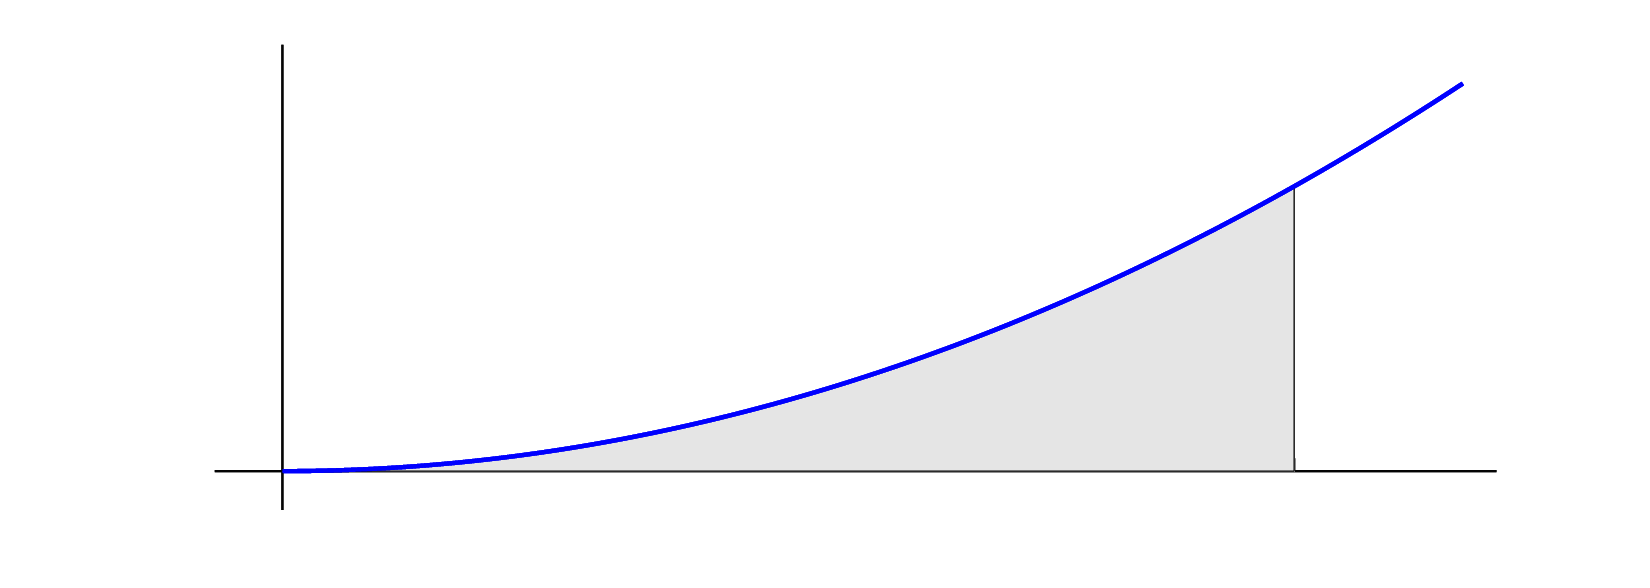
\includegraphics[width=14cm,height=5cm]{fig_area_x2}
\end{picture}%
\begin{picture}(396,141)(0,0)
\fontsize{10}{0}\selectfont\put(310.588,20.5695){\makebox(0,0)[t]{\textcolor[rgb]{0.15,0.15,0.15}{{$b$}}}}
\fontsize{10}{0}\selectfont\put(359.15,126.763){\makebox(0,0)[l]{\textcolor[rgb]{0,0,0}{{$y=x^2$}}}}
\end{picture}

\end{frame}

%------------------------------------------------------------------------------%
\begin{frame}{Aproximando a área sob o gráfico}
  \centering
  \vspace{1.6\baselineskip}
  % Title: Figure 1
% Creator: GL2PS 1.4.2, (C) 1999-2020 C. Geuzaine
% For: Octave
% CreationDate: Fri Aug  4 14:08:21 2023
\setlength{\unitlength}{1pt}
\begin{picture}(0,0)
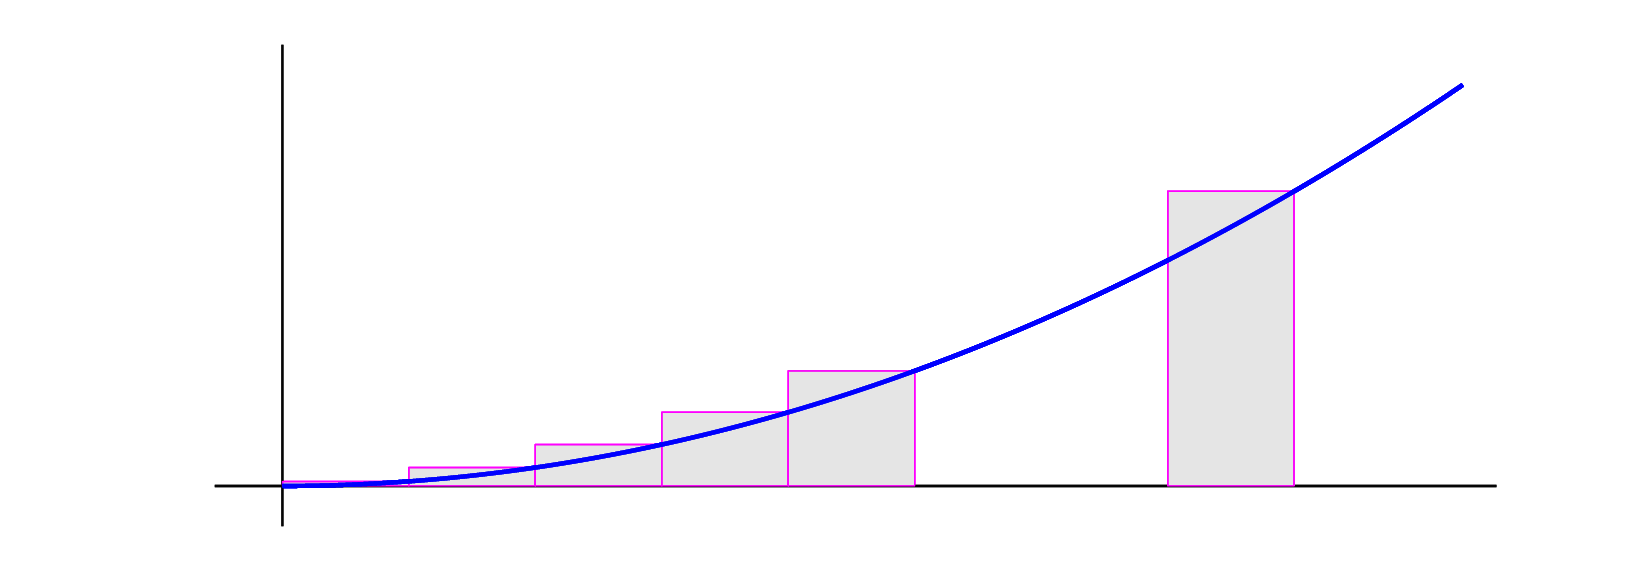
\includegraphics[width=14cm,height=5cm]{fig_area_x2_retangulos}
\end{picture}%
\begin{picture}(396,141)(0,0)
\fontsize{10}{0}\selectfont\put(359.15,126.638){\makebox(0,0)[l]{\textcolor[rgb]{0,0,0}{{$y=x^2$}}}}
\fontsize{10}{0}\selectfont\put(102.176,9.55416){\makebox(0,0)[b]{\textcolor[rgb]{0,0,0}{{$x_1$}}}}
\fontsize{10}{0}\selectfont\put(132.527,9.55416){\makebox(0,0)[b]{\textcolor[rgb]{0,0,0}{{$x_2$}}}}
\fontsize{10}{0}\selectfont\put(162.878,9.55416){\makebox(0,0)[b]{\textcolor[rgb]{0,0,0}{{$x_3$}}}}
\fontsize{10}{0}\selectfont\put(193.23,9.55416){\makebox(0,0)[b]{\textcolor[rgb]{0,0,0}{{$x_4$}}}}
\fontsize{10}{0}\selectfont\put(223.581,9.55416){\makebox(0,0)[b]{\textcolor[rgb]{0,0,0}{{$x_5$}}}}
\fontsize{10}{0}\selectfont\put(253.932,9.55416){\makebox(0,0)[b]{\textcolor[rgb]{0,0,0}{{$\cdots$}}}}
\fontsize{10}{0}\selectfont\put(284.283,9.55416){\makebox(0,0)[b]{\textcolor[rgb]{0,0,0}{{$x_{n-1}$}}}}
\fontsize{10}{0}\selectfont\put(322.728,9.55416){\makebox(0,0)[b]{\textcolor[rgb]{0,0,0}{{$b=x_n$}}}}
\fontsize{10}{0}\selectfont\put(76.6809,27.6274){\makebox(0,0)[bl]{\textcolor[rgb]{0,0,0}{{$A_1$}}}}
\fontsize{10}{0}\selectfont\put(110.27,32.6614){\makebox(0,0)[bl]{\textcolor[rgb]{0,0,0}{{$A_2$}}}}
\fontsize{10}{0}\selectfont\put(140.621,37.5481){\makebox(0,0)[bl]{\textcolor[rgb]{0,0,0}{{$A_3$}}}}
\fontsize{10}{0}\selectfont\put(170.972,46.2164){\makebox(0,0)[bl]{\textcolor[rgb]{0,0,0}{{$A_4$}}}}
\fontsize{10}{0}\selectfont\put(201.323,56.3089){\makebox(0,0)[bl]{\textcolor[rgb]{0,0,0}{{$A_5$}}}}
\fontsize{10}{0}\selectfont\put(292.377,97.4895){\makebox(0,0)[bl]{\textcolor[rgb]{0,0,0}{{$A_n$}}}}
\end{picture}

\end{frame}

%------------------------------------------------------------------------------%
\begin{frame}{Aproximando a área sob o gráfico}
Partição do intervalo $[0, b]$ em $n$ subintervalos iguais
\[
  0 = x_0 < x_1 < x_2 < \cdots < x_{n-1} < x_n = b
\]
\pause
Tamanho de cada subintervalo
\[
  \Delta x
  = x_{i+1} - x_i
  \pause
  = \frac{b}{n}
\]
\pause
Valor de $x_i$
\[
  x_i
  = i \Delta x
  \pause
  = i\frac{b}{n}
\]
\pause
Área de cada retângulo
\[
  A_i
  = x_i^2 \Delta x
  \pause
  = \left(i\frac{b}{n}\right)^2 \frac{b}{n}
  \pause
  = \frac{b^3}{n^3}i^2
\]
\end{frame}

%------------------------------------------------------------------------------%
\begin{frame}{Somando os Retângulos}
\begin{align*}
  \onslide<+->{ \tilde{A}_n & = \sum_{i=1}^n A_i }
  \onslide<+->{ \;=\; \sum_{i=1}^n \frac{b^3}{n^3}i^2               }
  \onslide<+->{ \;=\; \frac{b^3}{n^3} \sum_{i=1}^n i^2             \\[5mm]}
  \onslide<+->{ & = \frac{b^3}{n^3} \; \frac{n(n+1)(2n+1)}{6}      \\[5mm]}
  \onslide<+->{ & = \frac{b^3}{n^3} \; \frac{2n^3+3n^2+n}{6}       \\[5mm]}
  \onslide<+->{ & = \frac{b^3}{6} \left( 2+\frac{3}{n}+\frac{1}{n^2} \right) }
\end{align*}
\end{frame}

%------------------------------------------------------------------------------%
\begin{frame}{Calculando pelo limite}
  \begin{align*}
    \onslide<+->{ A & = \lim_{n\to\infty} \tilde{A}_n                   \\[7mm]}
    \onslide<+->{   & = \lim_{n\to\infty}
                        \frac{b^3}{6}
                        \left( 2+\frac{3}{n}+\frac{1}{n^2} \right)       \\[7mm]}
    \onslide<+->{   & = \frac{b^3}{6}
                        \left( 2 + 3 \lim_{n\to\infty} \frac{1}{n}
                                 +   \lim_{n\to\infty} \frac{1}{n^2} \right) \\[7mm]}
    \onslide<+->{   & = \frac{b^3}{6} 2 \;=\; \frac{b^3}{3}}
  \end{align*}
\end{frame}

%------------------------------------------------------------------------------%
\begin{frame}{Área entre o gráfico de $f$ e o eixo $x$ no intervalo $[a, b]$}
  \centering
  \vspace{2.3\baselineskip}
  \input{fig_integral_definida_area}
\end{frame}

%------------------------------------------------------------------------------%
\begin{frame}{Partição do intervalo $[a, b]$}
  \centering
  \vspace{2\baselineskip}
  % Title: Figure 1
% Creator: GL2PS 1.4.2, (C) 1999-2020 C. Geuzaine
% For: Octave
% CreationDate: Fri Aug  4 13:37:02 2023
\setlength{\unitlength}{1pt}
\begin{picture}(0,0)
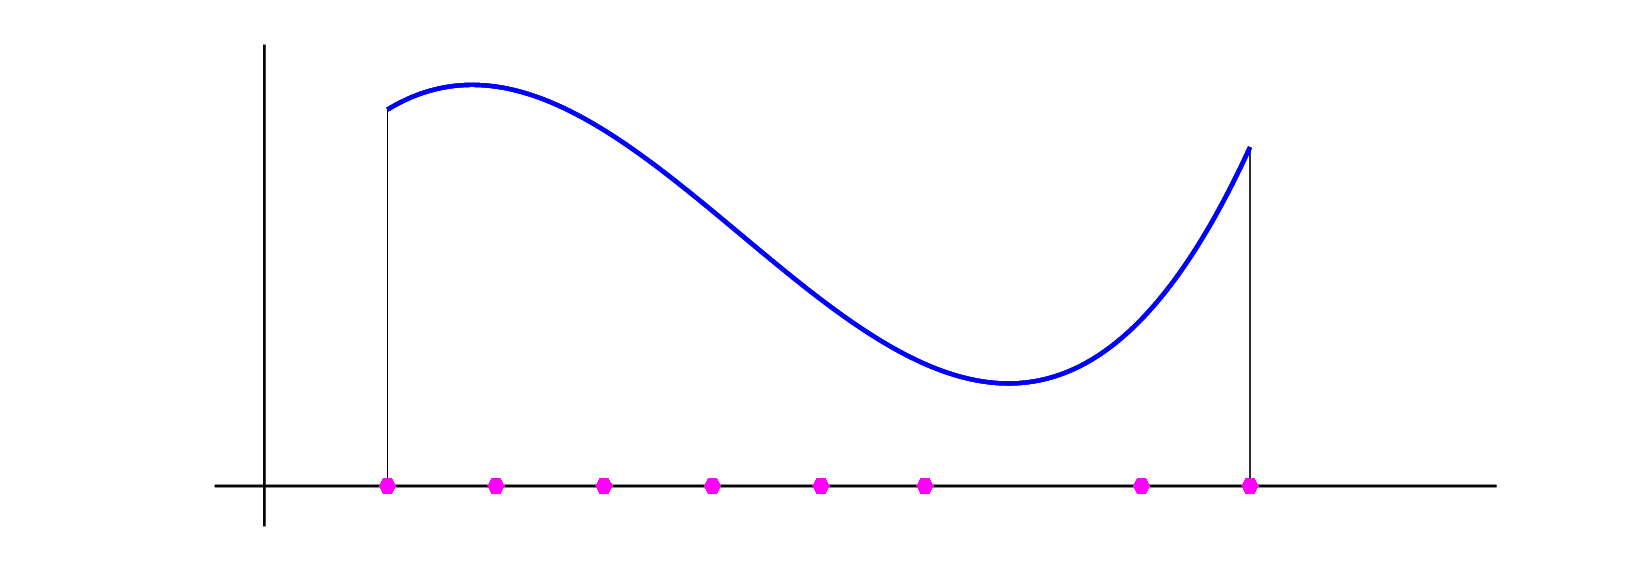
\includegraphics[width=14cm,height=5cm]{fig_soma_riemman_particao}
\end{picture}%
\begin{picture}(396,141)(0,0)
\fontsize{10}{0}\selectfont\put(311.833,109.399){\makebox(0,0)[l]{\textcolor[rgb]{0,0,0}{{$y=f(x)$}}}}
\fontsize{10}{0}\selectfont\put(93.5842,8.22396){\makebox(0,0)[b]{\textcolor[rgb]{0,0,0}{{$a=x_0$}}}}
\fontsize{10}{0}\selectfont\put(121.956,8.22396){\makebox(0,0)[b]{\textcolor[rgb]{0,0,0}{{$x_1$}}}}
\fontsize{10}{0}\selectfont\put(147.963,8.22396){\makebox(0,0)[b]{\textcolor[rgb]{0,0,0}{{$x_2$}}}}
\fontsize{10}{0}\selectfont\put(173.969,8.22396){\makebox(0,0)[b]{\textcolor[rgb]{0,0,0}{{$x_3$}}}}
\fontsize{10}{0}\selectfont\put(199.976,8.22396){\makebox(0,0)[b]{\textcolor[rgb]{0,0,0}{{$x_4$}}}}
\fontsize{10}{0}\selectfont\put(224.942,8.22396){\makebox(0,0)[b]{\textcolor[rgb]{0,0,0}{{$x_5$}}}}
\fontsize{10}{0}\selectfont\put(250.948,8.22396){\makebox(0,0)[b]{\textcolor[rgb]{0,0,0}{{$\cdots$}}}}
\fontsize{10}{0}\selectfont\put(276.955,8.22396){\makebox(0,0)[b]{\textcolor[rgb]{0,0,0}{{$x_{n-1}$}}}}
\fontsize{10}{0}\selectfont\put(307.693,8.22396){\makebox(0,0)[b]{\textcolor[rgb]{0,0,0}{{$b=x_n$}}}}
\end{picture}

\end{frame}

%------------------------------------------------------------------------------%
\begin{frame}{Aproximação por retângulos}
  \centering
  \vspace{2\baselineskip}
  % Title: Figure 1
% Creator: GL2PS 1.4.2, (C) 1999-2020 C. Geuzaine
% For: Octave
% CreationDate: Fri Aug  4 13:37:03 2023
\setlength{\unitlength}{1pt}
\begin{picture}(0,0)
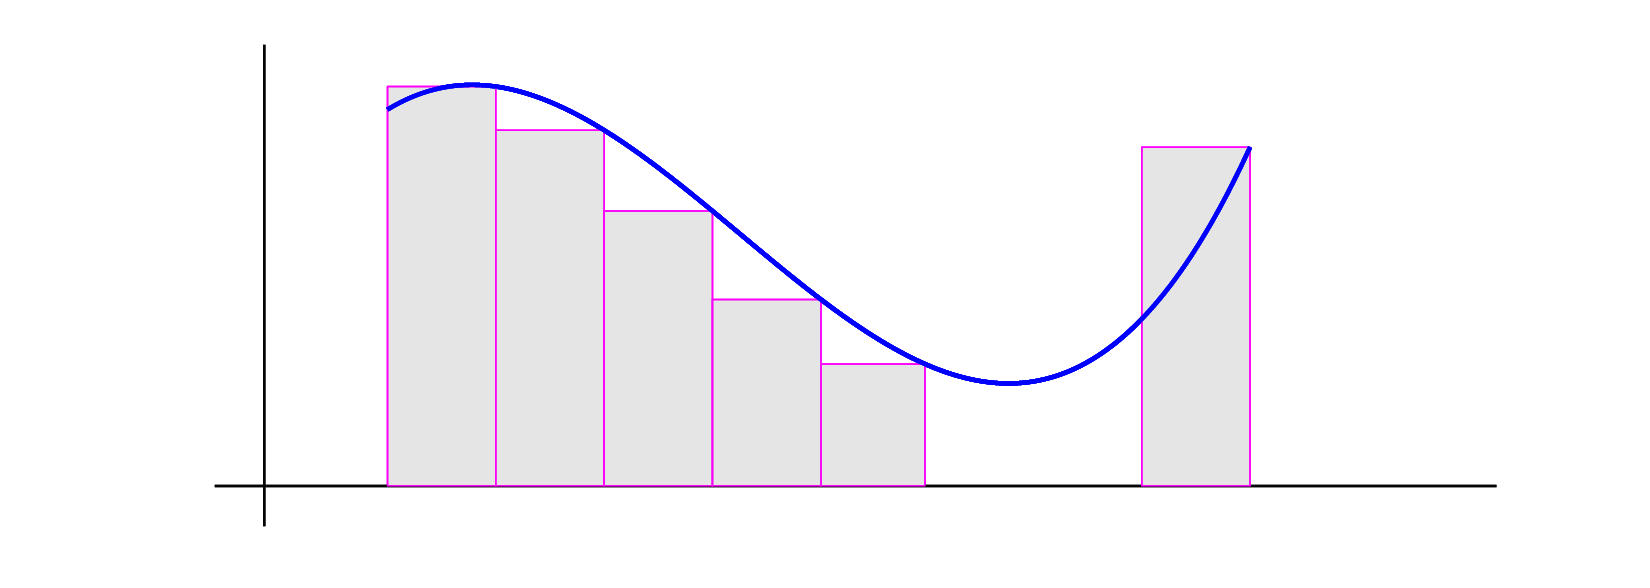
\includegraphics[width=14cm,height=5cm]{fig_soma_riemman_retangulos}
\end{picture}%
\begin{picture}(396,141)(0,0)
\fontsize{10}{0}\selectfont\put(311.833,109.399){\makebox(0,0)[l]{\textcolor[rgb]{0,0,0}{{$y=f(x)$}}}}
\fontsize{10}{0}\selectfont\put(93.5842,8.22396){\makebox(0,0)[b]{\textcolor[rgb]{0,0,0}{{$a=x_0$}}}}
\fontsize{10}{0}\selectfont\put(121.956,8.22396){\makebox(0,0)[b]{\textcolor[rgb]{0,0,0}{{$x_1$}}}}
\fontsize{10}{0}\selectfont\put(147.963,8.22396){\makebox(0,0)[b]{\textcolor[rgb]{0,0,0}{{$x_2$}}}}
\fontsize{10}{0}\selectfont\put(173.969,8.22396){\makebox(0,0)[b]{\textcolor[rgb]{0,0,0}{{$x_3$}}}}
\fontsize{10}{0}\selectfont\put(199.976,8.22396){\makebox(0,0)[b]{\textcolor[rgb]{0,0,0}{{$x_4$}}}}
\fontsize{10}{0}\selectfont\put(224.942,8.22396){\makebox(0,0)[b]{\textcolor[rgb]{0,0,0}{{$x_5$}}}}
\fontsize{10}{0}\selectfont\put(250.948,8.22396){\makebox(0,0)[b]{\textcolor[rgb]{0,0,0}{{$\cdots$}}}}
\fontsize{10}{0}\selectfont\put(276.955,8.22396){\makebox(0,0)[b]{\textcolor[rgb]{0,0,0}{{$x_{n-1}$}}}}
\fontsize{10}{0}\selectfont\put(307.693,8.22396){\makebox(0,0)[b]{\textcolor[rgb]{0,0,0}{{$b=x_n$}}}}
\fontsize{10}{0}\selectfont\put(99.4988,35.3245){\makebox(0,0)[bl]{\textcolor[rgb]{0,0,0}{{$A_1$}}}}
\fontsize{10}{0}\selectfont\put(127.871,35.3245){\makebox(0,0)[bl]{\textcolor[rgb]{0,0,0}{{$A_2$}}}}
\fontsize{10}{0}\selectfont\put(153.877,35.3245){\makebox(0,0)[bl]{\textcolor[rgb]{0,0,0}{{$A_3$}}}}
\fontsize{10}{0}\selectfont\put(179.884,35.3245){\makebox(0,0)[bl]{\textcolor[rgb]{0,0,0}{{$A_4$}}}}
\fontsize{10}{0}\selectfont\put(205.89,35.3245){\makebox(0,0)[bl]{\textcolor[rgb]{0,0,0}{{$A_5$}}}}
\fontsize{10}{0}\selectfont\put(282.869,35.3245){\makebox(0,0)[bl]{\textcolor[rgb]{0,0,0}{{$A_n$}}}}
\end{picture}

\end{frame}

%------------------------------------------------------------------------------%
\begin{frame}{Aproximação por retângulos}
\begin{align*}
  \onslide<+->{\Delta x & = \frac{b-a}{n} \\[2mm]}
  \onslide<+->{x_i & = a + i\Delta x \\[3mm]}
  \onslide<+->{A_i & = f(x_i)\Delta x \\[8mm]}
  \onslide<+->{A & \approx A_1+A_2+A_3+\cdots+ A_n \\[2mm]}
  \onslide<+->{  & = f(x_1)\Delta x+ f(x_2) \Delta x+ f(x_3) \Delta x + \cdots + f(x_n)\Delta x}
\end{align*}
\end{frame}

%------------------------------------------------------------------------------%
\begin{frame}{Área via soma de Riemann}
  A \emph{área} da região sob o gráfico de uma \emph{função contínua} $f$
  no intervalo $[a, b]$\\
  é dada pelo limite.
  \[
    A = \lim_{n \to \infty} \; \sum_{i=1}^n f(x_i) \Delta x
  \]
\end{frame}

%------------------------------------------------------------------------------%
\begin{frame}{Definição Integral Definida}
  A \emph{Integral Definida} de $f$ de $a$ até $b$ é
  \[
    \int_a^b f(x) dx
    \;=\; \lim_{n \to \infty} \; \sum_{i=1}^n f(c_i) \Delta x
  \]
  Desde que esse limite exista.

  \vspace{\baselineskip}
  $c_i\in[x_{i-1}, x_i]$ são os \emph{pontos amostrais}
\end{frame}

%------------------------------------------------------------------------------%
\begin{frame}{Consequência da Definição}
  A área tem o mesmo \emph{sinal} da função

  \begin{center}
    
\includegraphics[height=5cm]{integral_definida_03}
  \end{center}
\end{frame}

%------------------------------------------------------------------------------%
\section{Propriedades da integral definida}

%------------------------------------------------------------------------------%
\begin{frame}{Sentido de integração}
  \Large
  \[
    \int_{\textcolor{blue}{a}}^{\textcolor{magenta}{b}} f(x)\,dx
    = \textcolor{red}{-}
    \int^{\textcolor{blue}{a}}_{\textcolor{magenta}{b}} f(x)\,dx
  \]
\end{frame}

%------------------------------------------------------------------------------%
\begin{frame}{Intervalo de comprimento nulo}
  \Large
  \[
    \int_{\textcolor{blue}{a}}^{\textcolor{blue}{a}} f(x)dx
    = \textcolor{blue}{0}
  \]
\end{frame}

%------------------------------------------------------------------------------%
\begin{frame}{Área de um retângulo}{}
  {\Large
  \[
    \int_{a}^b {\color{blue}c}\,dx = {\color{blue}c}(b-a)
  \]}
  {\color{blue}$c$} constante
\end{frame}

%------------------------------------------------------------------------------%
\begin{frame}{Soma e subtração de funções}
  \Large
  \[
    \int_{a}^b \big[ f(x) \;{\color{blue}+}\; g(x) \big] dx
    = \int_{a}^b f(x)\,dx \;{\color{blue}+}\, \int_{a}^b g(x)\,dx
  \]
  ~
  \[
    \int_{a}^b \big[ f(x) \;{\color{blue}-}\; g(x) \big] dx
    = \int_{a}^b f(x)\,dx \;{\color{blue}-}\, \int_{a}^b g(x)\,dx
  \]
\end{frame}

%------------------------------------------------------------------------------%
\begin{frame}{Multiplicação de função por constante}{}
  {\Large
  \[
    \int_{a}^b \textcolor{blue}{c}\,f(x)\,dx
    = \textcolor{blue}{c} \int_{a}^b f(x)\,dx
  \]}
  ~

  \textcolor{blue}{$c$} constante
\end{frame}

%------------------------------------------------------------------------------%
\begin{frame}{Separando o intervalo em dois}
  \Large
  \[
    \int_{\textcolor{blue}{a}}^{\textcolor{blue}{b}} f(x)\,dx
    = \int_{\textcolor{blue}{a}}^{\textcolor{magenta}{c}} f(x)\,dx
    + \int_{\textcolor{magenta}{c}}^{\textcolor{blue}{b}} f(x)\,dx
  \]
\end{frame}

%------------------------------------------------------------------------------%
\begin{frame}{Área positiva}
  \Large
  Se \(f(x)\textcolor{blue}{\,\geq\,} 0\) para \(a \leq x \leq b\), então
  \(
    \int_{a}^b f(x)\,dx \textcolor{blue}{\,\geq\,} 0
  \)
\end{frame}

%------------------------------------------------------------------------------%
\begin{frame}{Comparação entre áreas}
  \Large
  Se \textcolor{blue}{$f(x) \geq g(x)$}
  para $a \leq x \leq b$, então \\[9mm]
  \[
    \int_{a}^b f(x)\,dx \;\textcolor{blue}{\,\geq\,}\; \int_{a}^b g(x)\,dx
  \]
\end{frame}

%------------------------------------------------------------------------------%
\begin{frame}{Limitação inferior e superior}
  \Large
  Se {${\color{blue}m} \leq f(x) \leq {\color{red}M}$} para $a \leq x \leq b$ então \\[9mm]
  \[
    {\color{blue} m}(b-a)                 \quad\geq\quad
    \int_{a}^b f(x)\,dx    \quad\geq\quad
    {\color{red} M}(b-a)
  \]
\end{frame}

%------------------------------------------------------------------------------%
\begin{frame}
  \tableofcontents
\end{frame}

%------------------------------------------------------------------------------%
\end{document}
%------------------------------------------------------------------------------%
